\documentclass{beamer}
\usetheme{metropolis}
\usepackage{../../resources/style}
\usetikzlibrary{trees}

\newcommand{\beginnote}[1]{%
  \vfill
  {\footnotesize\textcolor{gray}{\textit{$\triangleright$ #1 (vezi slide-ul \emph{Resurse})}}}%
}

\title{Șirul lui Fibonacci | Algoritmi pe șiruri}
\subtitle{Elementul majoritar $\cdot$ Subsecvența de sumă maximă}
\author{Andrei Mihai Ciobanu}
\institute{Algolymp Summer School}
\date{}
\titlegraphic{
\includegraphics[width=4cm]{../../resources/algolymp-logo.png}}
\setbeamertemplate{frame footer}{Algolymp Summer School}

% ----------------------------------------------------------------
\begin{document}

\begin{frame}[shrink]
  \titlepage
\end{frame}

\begin{frame}{Cuprins}
  \tableofcontents
\end{frame}

% ================================================================
\section{Șirul lui Fibonacci}

\begin{frame}{Definiție și recurență}
  \begin{block}{Șirul lui Fibonacci}
    \[
      F[0] = 0, \quad F[1] = 1, \quad F[i] = F[i-1] + F[i-2] \text{ pentru } i \geq 2
    \]
  \end{block}

  \smallskip
  \begin{center}
  \begin{tabular}{lccccccccc}
    \toprule
    $i$    & 0 & 1 & 2 & 3 & 4 & 5 & 6 & 7 & 8 \\
    \midrule
    $F[i]$ & 0 & 1 & 1 & 2 & 3 & 5 & 8 & 13 & 21 \\
    \bottomrule
  \end{tabular}
  \end{center}

  \smallskip
  Fiecare termen e suma celor doi dinaintea lui. Întrebarea cheie: ca să calculăm $F[i]$, de ce informație avem \textbf{cu adevărat} nevoie?
\end{frame}

\begin{frame}[fragile]{Varianta recursivă naivă}
  \begin{lstlisting}
long long fibonacci(int n) {
    if (n < 2) {
        return n;
    }
    return fibonacci(n - 1) + fibonacci(n - 2);
}
  \end{lstlisting}
  \begin{itemize}
    \item Codul arată exact ca formula, dar e \textbf{foarte lent}.
    \item Problema: aceleași subprobleme se \textbf{recalculează de mai multe ori} \textemdash{} \lstinline|fibonacci(2)| e recalculat ori de câte ori e nevoie de el.
    \item \lstinline|fibonacci(40)| face $\approx 330$ de milioane de apeluri; \lstinline|fibonacci(100)| nu se termină în timp rezonabil.
  \end{itemize}
\end{frame}

\begin{frame}{Arborele de apeluri \textemdash{} fibonacci(3)}
  \begin{center}
  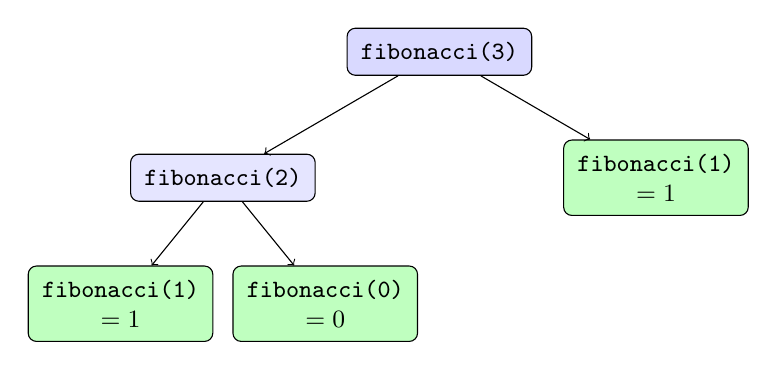
\begin{tikzpicture}[
    level distance=1.6cm,
    level 1/.style={sibling distance=5.5cm},
    level 2/.style={sibling distance=2.6cm},
    edge from parent/.style={draw, ->},
    every node/.style={draw, rounded corners=3pt, fill=gray!10,
                        font=\small, inner sep=5pt, align=center}
  ]
  \node[fill=blue!15] {\texttt{fibonacci(3)}}
    child { node[fill=blue!10] {\texttt{fibonacci(2)}}
      child { node[fill=green!25] {\texttt{fibonacci(1)}\\\small$= 1$} }
      child { node[fill=green!25] {\texttt{fibonacci(0)}\\\small$= 0$} }
    }
    child { node[fill=green!25] {\texttt{fibonacci(1)}\\\small$= 1$} };
  \end{tikzpicture}
  \end{center}
  \smallskip
  Fiecare nod non-terminal generează exact 2 apeluri recursive. Total: \textbf{5 apeluri} pentru $n = 3$.
\end{frame}

\begin{frame}{Arborele de apeluri \textemdash{} fibonacci(5)}
  \begin{center}
  \resizebox{\linewidth}{!}{%
  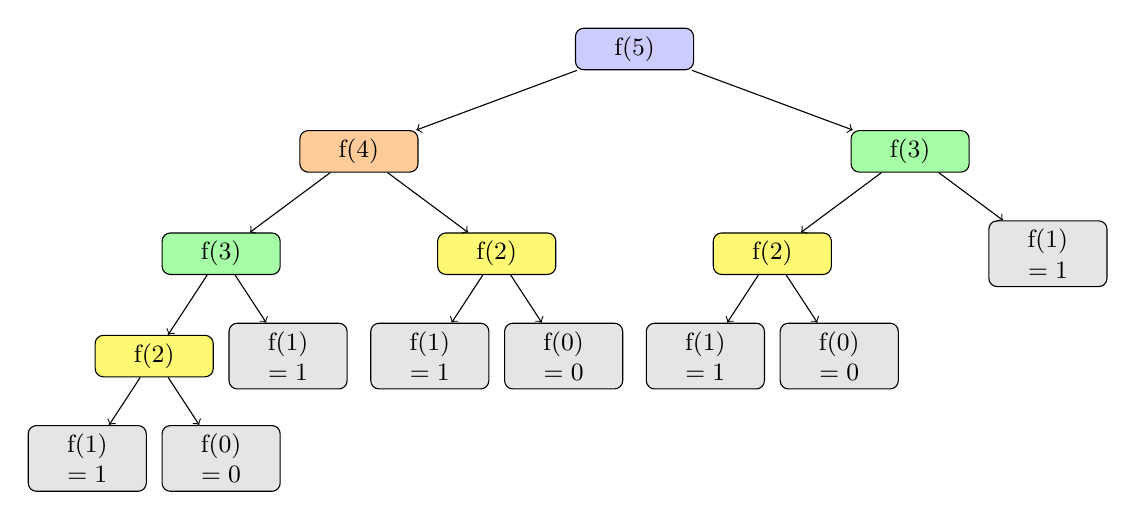
\begin{tikzpicture}[
    level distance=1.3cm,
    level 1/.style={sibling distance=7cm},
    level 2/.style={sibling distance=3.5cm},
    level 3/.style={sibling distance=1.7cm},
    edge from parent/.style={draw, ->, thin},
    every node/.style={draw, rounded corners=3pt, font=\small,
                        inner sep=3pt, minimum width=1.5cm, align=center}
  ]
  \node[fill=blue!20] {f(5)}
    child { node[fill=orange!40] {f(4)}
      child { node[fill=green!35] {f(3)}
        child { node[fill=yellow!55] {f(2)}
          child { node[fill=gray!20] {f(1)\\$=1$} }
          child { node[fill=gray!20] {f(0)\\$=0$} }
        }
        child { node[fill=gray!20] {f(1)\\$=1$} }
      }
      child { node[fill=yellow!55] {f(2)}
        child { node[fill=gray!20] {f(1)\\$=1$} }
        child { node[fill=gray!20] {f(0)\\$=0$} }
      }
    }
    child { node[fill=green!35] {f(3)}
      child { node[fill=yellow!55] {f(2)}
        child { node[fill=gray!20] {f(1)\\$=1$} }
        child { node[fill=gray!20] {f(0)\\$=0$} }
      }
      child { node[fill=gray!20] {f(1)\\$=1$} }
    };
  \end{tikzpicture}
  }
  \end{center}
  \vspace{-4pt}
  Total: \textbf{15 apeluri}. Noduri de aceeași culoare = calcule repetate.
\end{frame}

\begin{frame}{Câte apeluri face fibonacci(n)?}
  \begin{center}
  \begin{tabular}{lcccccccccc}
    \toprule
    $n$       & 1 & 2 & 3 & 4 & 5  & 6  & 7  & 8  & 9   & 10  \\
    \midrule
    $F[n]$    & 1 & 1 & 2 & 3 & 5  & 8  & 13 & 21 & 34  & 55  \\
    Apeluri   & 1 & 3 & 5 & 9 & 15 & 25 & 41 & 67 & 109 & 177 \\
    \bottomrule
  \end{tabular}
  \end{center}

  \smallskip
  Observăm că numărul de apeluri pentru $n$ este exact $2 \cdot F[n+1] - 1$.

  \smallskip
  Numărul de apeluri crește \textbf{mult mai rapid} decât valorile Fibonacci $\rightarrow$ creștere exponențială.
\end{frame}

\begin{frame}{Creștere exponențială și golden ratio ($\varphi$)}
  Dacă împărțim numărul de apeluri de la $x$ la cel de la $x-1$:

  \smallskip
  \begin{center}
  \begin{tabular}{cc}
    \toprule
    $x$ & apeluri$(x)$ / apeluri$(x-1)$ \\
    \midrule
    3  & $5\,/\,3   \approx 1{,}67$ \\
    5  & $15\,/\,9  \approx 1{,}67$ \\
    7  & $41\,/\,25 \approx 1{,}64$ \\
    9  & $109\,/\,67  \approx 1{,}63$ \\
    10 & $177\,/\,109 \approx 1{,}62$ \\
    \bottomrule
  \end{tabular}
  \end{center}

  \smallskip
  Raportul se apropie de $\varphi \approx 1{,}618\ldots$ \textemdash{} \textbf{golden ratio}. Cu cât $x$ e mai mare, cu atât raportul converge mai precis.
\end{frame}

\begin{frame}{Fun fact: Numărul de aur și formula lui Binet}
  \begin{block}{Numărul de aur}
    \[
      \varphi = \frac{1 + \sqrt{5}}{2} \approx 1{,}618\ldots
    \]
  \end{block}

  \begin{block}{Formula lui Binet}
    \[
      F[n] = \frac{\varphi^n - \psi^n}{\sqrt{5}}, \quad \text{unde } \psi = \frac{1 - \sqrt{5}}{2} \approx -0{,}618
    \]
  \end{block}

  \begin{itemize}
    \item Deoarece $|\psi| < 1$, pentru $n$ mare: $F[n] \approx \varphi^n / \sqrt{5}$
    \item Asta explică de ce varianta recursivă naivă e $O(\varphi^n)$ \textemdash{} adică exponențială
    \item $\varphi$ apare și în natură: frunze, petale, spiralele scoicilor
  \end{itemize}
\end{frame}

\begin{frame}[fragile]{Varianta iterativă}
  Ca să calculăm $F[i]$, ne trebuie doar \textbf{ultimele două} valori: $F[i-2]$ și $F[i-1]$.
  \begin{lstlisting}
const long long MOD = 1000000007;

long long fibonacci(int t) {
    long long f0 = 0, f1 = 1;
    for (int i = 0; i < t; i++) {
        long long next = (f0 + f1) % MOD;
        f0 = f1;
        f1 = next;
    }
    return f0;
}
  \end{lstlisting}
  După $i$ pași, \lstinline|f0| memorează $F[i]$ \textemdash{} de aceea, după $t$ pași, \lstinline|f0| este exact $F[t]$.
\end{frame}

\begin{frame}{Complexitate \textemdash{} Fibonacci}
  \begin{center}
  \begin{tabular}{lll}
    \toprule
    Variantă & Timp & Spațiu \\
    \midrule
    Recursivă naivă & $O(\varphi^n)$ & $O(n)$ (stivă) \\
    Iterativă        & $O(t)$        & $O(1)$ \\
    \bottomrule
  \end{tabular}
  \end{center}

  \smallskip
  \begin{block}{Bonus}
    Dacă $t$ e extrem de mare (ex. $10^{18}$), există metode $O(\log t)$ prin \textbf{exponențiere matriceală} sau \textit{fast doubling}. Nu sunt necesare acum, dar ideea de înjumătățire va reapărea.
  \end{block}
\end{frame}

% ================================================================
\section{Elementul majoritar}

\begin{frame}{Ce este un element majoritar?}
  \begin{block}{Element majoritar strict}
    O valoare care apare de \textbf{mai mult de} $n/2$ ori într-un șir cu $n$ elemente.
  \end{block}

  \smallskip
  Exemplu: $v = [7, 2, 7, 7, 4]$ \textemdash{} valoarea $7$ apare de $3$ ori din $5$, deci este majoritar ($3 > 5/2$).

  \smallskip
  Contraexemplu: $v = [1, 1, 2, 2]$ \textemdash{} cele mai frecvente valori apar de $2$ ori, dar $2$ nu e mai mare decât $4/2$, deci \textbf{nu există} element majoritar.

  \smallskip
  \begin{block}{Atenție}
    ``Cea mai frecventă valoare'' \textbf{nu} este același lucru cu ``element majoritar strict''.
  \end{block}
\end{frame}

\begin{frame}{Povestea voturilor}
  Imaginați-vă o alegere: $n$ votanți, fiecare votează un candidat. Un candidat câștigă dacă primește \textbf{mai mult de jumătate} din voturi \textemdash{} adică are \textbf{majoritate absolută}.

  \smallskip
  \begin{block}{Regula de anulare}
    Oricare doi votanți care au votat candidați \textbf{diferiți} se anulează reciproc și ies amândoi din joc.
  \end{block}

  \smallskip
  \begin{itemize}
    \item Dacă există un candidat majoritar, are prea mulți susținători pentru a fi anulat complet \textemdash{} vor rămâne mereu unii care l-au votat
    \item Dacă \textbf{nu} există majoritar, e posibil ca toți să se anuleze
    \item La final, candidatul rămas este un \textbf{candidat posibil} \textemdash{} nu neapărat câștigător, trebuie verificat!
  \end{itemize}
\end{frame}

\begin{frame}{Traseu pas cu pas \textemdash{} $v = [7, 2, 7, 7, 4]$}
  \begin{center}
  \begin{tabular}{cccc}
    \toprule
    $i$ & $v[i]$ & \texttt{candidat} & \texttt{voturi} \\
    \midrule
    \textemdash{} & \textemdash{} & \textemdash{} & 0 \\
    0 & 7 & 7 & 1 \\
    1 & 2 & 7 & 0 \\
    2 & 7 & 7 & 1 \\
    3 & 7 & 7 & 2 \\
    4 & 4 & 7 & 1 \\
    \bottomrule
  \end{tabular}
  \end{center}

  \smallskip
  Reguli: \texttt{voturi}$=0$ $\Rightarrow$ candidat nou; $v[i] =$ \texttt{candidat} $\Rightarrow$ \texttt{voturi++}; altfel $\Rightarrow$ \texttt{voturi\textendash{}\textendash{}}.

  \smallskip
  Candidat final: \textbf{7}. Urmează pasul de verificare.
\end{frame}

\begin{frame}{Ideea de anulare}
  Imaginăm că împerechem valori diferite și le ștergem pe rând:

  \smallskip
  $v = [7, 2, 7, 7, 4]$

  \begin{itemize}
    \item Ștergem $7$ cu $2$: rămâne $[7, 7, 4]$
    \item Ștergem $7$ cu $4$: rămâne $[7]$
  \end{itemize}

  \smallskip
  Dacă o valoare apare de mai mult de jumătate din numărul total de ori, ea \textbf{nu poate dispărea complet} \textemdash{} are prea mulți reprezentanți.

  \smallskip
  Algoritmul lui \textbf{Boyer-Moore} implementează exact această idee eficient, fără să memoreze efectiv perechile.
\end{frame}

\begin{frame}[fragile]{Algoritmul Boyer-Moore}
  \begin{lstlisting}
int candidat = 0;
int voturi = 0;

for (int i = 0; i < n; i++) {
    int x = v[i];
    if (voturi == 0) {
        candidat = x;
        voturi = 1;
    } else if (x == candidat) {
        voturi++;
    } else {
        voturi--;
    }
}
  \end{lstlisting}
  \lstinline|voturi| \textbf{nu} e frecvența reală, ci balanța rămasă după anulări. Codul de mai sus ne dă doar un \textbf{candidat}.
\end{frame}

\begin{frame}[fragile, shrink]{Pasul de verificare}
  De ce e necesară verificarea? Pentru $v = [1, 2, 3, 4, 5]$, Boyer-Moore tot termină cu un candidat \textemdash{} dar nicio valoare nu apare de mai mult de jumătate din numărul de ori.
  \begin{lstlisting}
int frecventa = 0;
for (int i = 0; i < n; i++) {
    if (v[i] == candidat) {
        frecventa++;
    }
}

if (frecventa > n / 2) {
    cout << candidat;
} else {
    cout << -1;
}
  \end{lstlisting}
  \textbf{Cel mai frecvent bug:} uitarea pasului de verificare. Condiția este \textbf{strict} mai mare decât $n/2$.
\end{frame}

\begin{frame}{Complexitate \textemdash{} Element majoritar}
  \begin{center}
  \begin{tabular}{lll}
    \toprule
    Etapă & Timp & Spațiu \\
    \midrule
    Găsire candidat (Boyer-Moore) & $O(n)$ & $O(1)$ \\
    Verificare candidat           & $O(n)$ & $O(1)$ \\
    \midrule
    \textbf{Total}                & $O(n)$ & $O(1)$ \\
    \bottomrule
  \end{tabular}
  \end{center}

  \smallskip
  Mult mai rapid decât abordarea naivă (numărare pentru fiecare valoare distinctă, $O(n^2)$ în cel mai rău caz).
\end{frame}

% ================================================================
\section{Subsecvența de sumă maximă}

\begin{frame}{Problema}
  \begin{block}{Cerință}
    Dat un șir de $n$ numere întregi (pot fi și negative), determinați suma maximă a unei \textbf{subsecvențe contigue} (elemente consecutive).
  \end{block}

  \smallskip
  Exemplu: $v = [-2, 1, -3, 4, -1, 2, 1, -5, 4]$

  \smallskip
  Subsecvența $[4, -1, 2, 1]$ are suma $6$ \textemdash{} aceasta este suma maximă posibilă.
\end{frame}

\begin{frame}[fragile]{Soluție naivă}
  \begin{lstlisting}
long long maxim = v[0];
for (int i = 0; i < n; i++) {
    long long suma = 0;
    for (int j = i; j < n; j++) {
        suma += v[j];
        maxim = max(maxim, suma);
    }
}
cout << maxim;
  \end{lstlisting}
  \begin{itemize}
    \item Încercăm \textbf{toate} subsecvențele posibile, calculând suma fiecăreia
    \item Complexitate: $O(n^2)$ \textemdash{} prea lent pentru $n$ mare
  \end{itemize}
\end{frame}

\begin{frame}[fragile]{Algoritmul lui Kadane}
  Pentru fiecare poziție, întrebarea e: continuăm subsecvența anterioară sau începem una nouă de aici?
  \begin{lstlisting}
long long sumaCurenta = v[0];
long long maxim = v[0];

for (int i = 1; i < n; i++) {
    sumaCurenta = max((long long)v[i], sumaCurenta + v[i]);
    maxim = max(maxim, sumaCurenta);
}
cout << maxim;
  \end{lstlisting}
  Dacă suma acumulată devine \textbf{mai mică} decât elementul curent, nu mai are sens s-o continuăm \textemdash{} pornim o subsecvență nouă.
\end{frame}

\begin{frame}{Complexitate \textemdash{} Subsecvența de sumă maximă}
  \begin{center}
  \begin{tabular}{lll}
    \toprule
    Variantă & Timp & Spațiu \\
    \midrule
    Naivă (toate subsecvențele) & $O(n^2)$ & $O(1)$ \\
    Kadane                      & $O(n)$   & $O(1)$ \\
    \bottomrule
  \end{tabular}
  \end{center}
\end{frame}

% ================================================================
\section{Recapitulare}

\begin{frame}{Recapitulare}
  \begin{center}
  \begin{tabular}{lll}
    \toprule
    Temă & Timp & Spațiu \\
    \midrule
    Fibonacci (iterativ)              & $O(t)$ & $O(1)$ \\
    Element majoritar (Boyer-Moore)   & $O(n)$ & $O(1)$ \\
    Subsecvența de sumă maximă (Kadane) & $O(n)$ & $O(1)$ \\
    \bottomrule
  \end{tabular}
  \end{center}

  \smallskip
  \begin{itemize}
    \item Fibonacci recursiv recalculează aceleași subprobleme \textemdash{} varianta iterativă rezolvă asta în $O(1)$ spațiu
    \item La elementul majoritar, un candidat găsit prin anulare \textbf{trebuie verificat}
    \item La Kadane, decizia la fiecare pas: continuăm sau pornim din nou
  \end{itemize}
\end{frame}

% ================================================================
\section{Resurse}

\begin{frame}{Resurse}
  \begin{block}{Șirul lui Fibonacci}
    \begin{itemize}\footnotesize\itemsep0pt
      \item \href{https://www.pbinfo.ro/articole/5537/sirul-lui-fibonacci}{\textbf{pbinfo.ro}} \textemdash{} Șirul lui Fibonacci (RO)
      \item \href{https://infoas.ro/lectie/105/sirul-lui-fibonacci-in-c}{\textbf{infoas.ro}} \textemdash{} Șirul lui Fibonacci în C++ (RO)
      \item \href{https://cp-algorithms.com/algebra/fibonacci-numbers.html}{\textbf{cp-algorithms.com}} \textemdash{} Fibonacci Numbers (EN, avansat)
      \item \href{https://en.wikipedia.org/wiki/Fibonacci_sequence}{\textbf{wikipedia.org}} \textemdash{} Fibonacci sequence (EN)
    \end{itemize}
  \end{block}
  \vspace{-6pt}
  \begin{block}{Elementul majoritar}
    \begin{itemize}\footnotesize\itemsep0pt
      \item \href{https://infoarena.ro/problema-majoritatii-votului}{\textbf{infoarena.ro}} \textemdash{} Problema majorității votului (RO)
      \item \href{https://tutoriale-pe.net/elementul-majoritar-elmaj/}{\textbf{tutoriale-pe.net}} \textemdash{} Elementul majoritar (RO)
      \item \href{https://www.geeksforgeeks.org/theory-of-computation/boyer-moore-majority-voting-algorithm/}{\textbf{geeksforgeeks.org}} \textemdash{} Boyer\textendash{}Moore Majority Voting (EN)
      \item \href{https://en.wikipedia.org/wiki/Boyer\%E2\%80\%93Moore_majority_vote_algorithm}{\textbf{wikipedia.org}} \textemdash{} Boyer\textendash{}Moore majority vote algorithm (EN)
    \end{itemize}
  \end{block}
  \vspace{-6pt}
  \begin{block}{Subsecvența de sumă maximă}
    \begin{itemize}\footnotesize\itemsep0pt
      \item \href{https://www.pbinfo.ro/articole/32848/algoritmul-lui-kadane}{\textbf{pbinfo.ro}} \textemdash{} Algoritmul lui Kadane (RO)
      \item \href{https://en.wikipedia.org/wiki/Maximum_subarray_problem}{\textbf{wikipedia.org}} \textemdash{} Maximum subarray problem (EN)
    \end{itemize}
  \end{block}
\end{frame}

% ================================================================
\section{Probleme de antrenament}

\begin{frame}{Probleme de antrenament}
  \begin{block}{Ușoare}
    \begin{itemize}\footnotesize\itemsep0pt
      \item \href{https://code.algolymp.com/problems/759}{\textbf{Fibonacci \#255 \#759}} {\footnotesize\textcolor{gray}{(AlgoCode)}}
      \item \href{https://code.algolymp.com/problems/4219}{\textbf{Majority Element \#4219}} {\footnotesize\textcolor{gray}{(AlgoCode)}}
    \end{itemize}
  \end{block}
  \vspace{-4pt}
  \begin{block}{Medie}
    \begin{itemize}\footnotesize\itemsep0pt
      \item \href{https://code.algolymp.com/problems/4362}{\textbf{Kadane Segment Report \#4362}} {\footnotesize\textcolor{gray}{(AlgoCode)}}
    \end{itemize}
  \end{block}
  \vspace{-4pt}
  \begin{block}{Olimpiadă}
    \begin{itemize}\footnotesize\itemsep0pt
      \item \href{https://code.algolymp.com/problems/226}{\textbf{avarcolaci}} {\footnotesize\textcolor{gray}{(ONI 2014, clasa XI\textendash{}XII)}}
    \end{itemize}
  \end{block}
\end{frame}

\end{document}
